\chapter{Evaluación y pruebas}\label{evaluacion}

En este capítulo se abordará la prueba del sistema. Para ello, a partir de un archivo que contenga una traza de tráfico, se procesará 
con el módulo creado, de forma que se compruebe que se crea el registro correspondiente y que este contiene los flujos emparejados.

\intro Se añadirán capturas de pantalla en las que se vea claramente que todo funciona como debería, así mismo, se podrán comprobar 
los registros que se creen en el repositorio de GitHub \citep{repo}.

\section{Establecer las variables}

Lo primero que se hará, será establecer las variables \textit{k1} y \textit{k2}. Estas se definen de forma global al principio 
del módulo. Cómo ya se vio anteriormente, ecuación \ref{ecug}, sus valores estarán comprendidos entre 0,1 y 10000. Como se puede ver 
en la Figura \ref{fig.variables}, para las pruebas se han establecido los valores en 1 y 100.

\begin{figure}[H]
  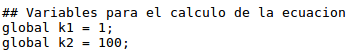
\includegraphics[width=0.6\textwidth]{imagenes/variables.png}
  \centering
  \caption{Valores de las variables \textit{k1 y k2}.}\label{fig.variables}
\end{figure}

\intro A su vez, también será necesario establecer el umbral que servirá para descartar o aceptar emparejamientos. Como se puede ver en la Figura \ref{fig.definirumbral}, en el caso de estas pruebas el valor será de 1.

\begin{figure}[H]
  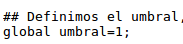
\includegraphics[width=0.3\textwidth]{imagenes/definirumbral.png}
  \centering
  \caption{Valor de la variable \textit{umbral}.}\label{fig.definirumbral}
\end{figure}


\section{Prueba del módulo}

A continuación, se realizará una prueba del módulo, con las variables anteriormente descritas, para comprobar que todo funciona 
correctamente.

\intro Como se puede ver en la Figura \ref{fig.terminal}, para lanzar el módulo, será necesario indicar el archivo que se va a 
analizar.

\begin{figure}[H]
  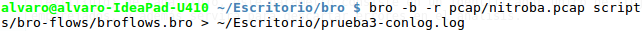
\includegraphics[width=0.9\textwidth]{imagenes/terminal.png}
  \centering
  \caption{Lanzamiento del módulo para realizar el análisis.}\label{fig.terminal}
\end{figure}

\intro En el registro que se crea cada vez que se ejecuta el análisis, además de las IP's y los puertos, también se muestran los 
\textit{uid} de cada flujo, este parámetro consiste en un identificador único de flujo. Esto ayudará a identificar los flujos que son 
emparejados, y además servirá para descartar errores en el análisis.

\intro En la Figura \ref{fig.lognitroba}, se puede comprobar el registro que se genera al analizar un archivo. En este caso el archivo 
analizado a sido \textit{nitroba.pcap}, cuyo peso es de 56,2 MB, el cual se encuentra accesible desde la web de Bro. Esta traza se 
corresponde con un escenario de prueba realizado por una universidad sudafricana. 

\begin{figure}[H]
  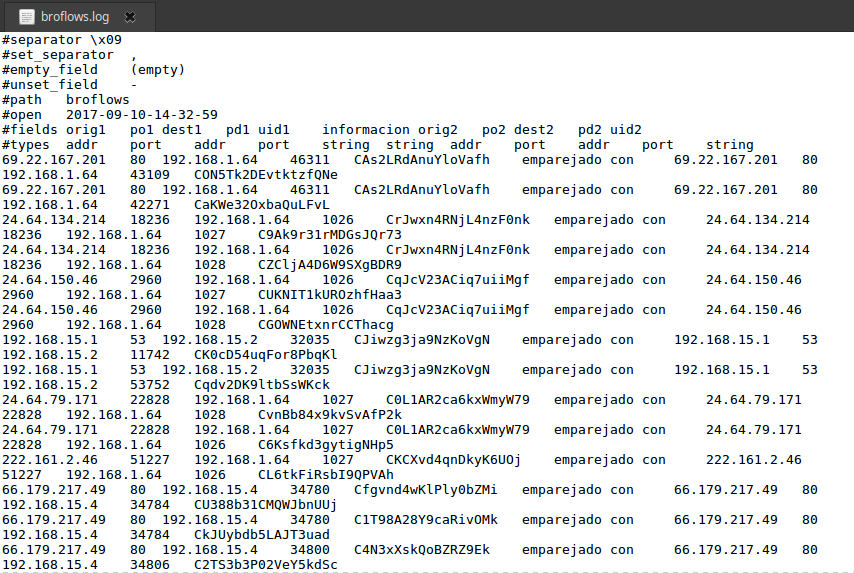
\includegraphics[width=0.9\textwidth]{imagenes/lognitroba.png}
  \centering
  \caption{Log del archivo \textit{nitroba.pcap}.}\label{fig.lognitroba}
\end{figure}

\intro Como se puede ver en \ref{fig.lognitroba}, los flujos son emparejados, por lo tanto se puede decir que el módulo funciona 
correctamente, al menos con trazas pequeñas. Este tipo de archivos son ideales para realizar las pruebas, pues tarda muy poco el 
sistema en analizarlos, siendo en este caso 1 segundo el tiempo utilizado.

\intro Además, no se entra dentro de los paquetes, por lo que la privacidad está garantizada.

\section{Escenarios reales}

Una vez que se ha comprobado que todo funciona como debe con un archivo pequeño, se pasará a analizar un archivo más grande, 
correspondiente a un escenario real. En este caso se trata de \textit{maccdc2012\_00004.pcap}, correspondiente al \textit{National 
CyberWatch Mid-Atlantic Collegiate Cyber Defense Competition} o \textit{MACCDC} \cite{maccdc}. En este se encuentra el tráfico de un 
día y ocupa cerca de 1.1 GB.

\intro En la Figura \ref{fig.logmaccdc} se puede ver que se trata de un registro mucho más extenso que el anterior. De hecho, tarda 
cerca de 50 minutos en realizar el análisis, frente al segundo que se tardaba con el anterior archivo.

\begin{figure}[H]
  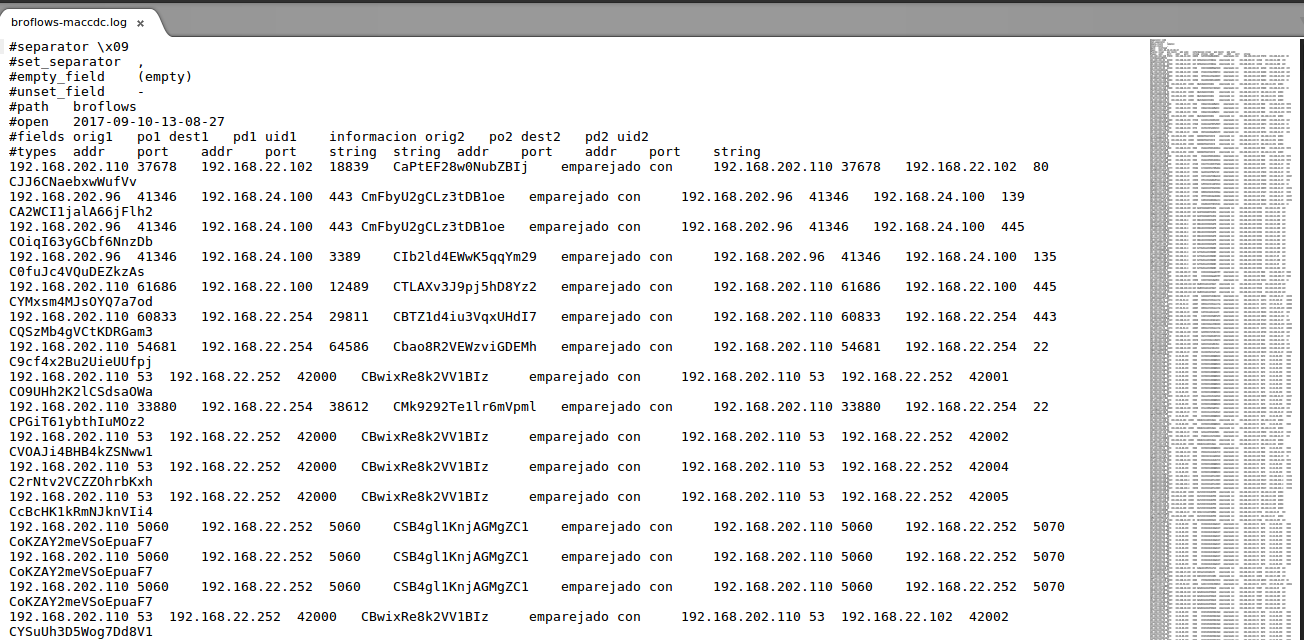
\includegraphics[width=1\textwidth]{imagenes/logmaccdc.png}
  \centering
  \caption{Log del archivo \textit{maccdc2012\_00004.pcap}.}\label{fig.logmaccdc}
\end{figure}

\intro En la Figura \ref{fig.flujosemparejados}, se puede comprobar cómo está almacenado distintos flujos, los cuales están 
emparejados con el mismo flujo activo, por lo que se tiene que todos esos flujos pertenecerán al mismo. Esta comprobación se puede 
realizar mediante los \textit{uids}, siendo el mismo para el primer flujo, o flujo activo, y distintos en los siguientes, por lo que 
van a IP's distintas o a puertos distintos, pero pertenecen al mismo flujo general de datos.

\begin{figure}[H]
  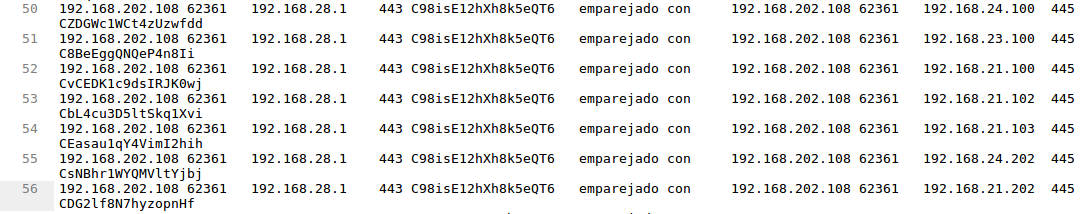
\includegraphics[width=1\textwidth]{imagenes/flujosemparejados.png}
  \centering
  \caption{Flujos emparejados.}\label{fig.flujosemparejados}
\end{figure}

\intro Si se realiza una búsqueda usando el \textit{uid} del primer flujo, se verá que no se muestra más veces, por lo que se realiza 
el borrado de la tabla de activos correctamente.

